\documentclass[10pt,journal,compsoc]{IEEEtran}

\usepackage[pdftex]{graphicx}    
\usepackage{cite}
\usepackage{caption}
\usepackage{subcaption}
\usepackage{mathtools}
\hyphenation{op-tical net-works semi-conduc-tor}
\graphicspath{ {../images/} }


\begin{document}

\title{Robotics Software Engineer Nanodegree: Localization Project}

\author{Manuel Huertas L\'opez}

\markboth{Localization project, Robotics Nanodegree Program, Udacity}%
{}
\IEEEtitleabstractindextext{%

\begin{abstract}
This project involves to accurately localize a mobile robot insided a provided map in Gazebo and RViz simulation enviroments. The goal includes to build a robot model in Gazebo and utilize packages like AMCL and the Navigation Stack to succefully identifed the position of the robot in the world. As a final test the robot will be commaned to a specific location and the navigation stack will determinate the route to follow. As part of the work it is neccessary to explore, add, and tunning specific parameters corresponding to each package to achieve the best possible localization result.
\end{abstract}


\begin{IEEEkeywords}
Robot, Udacity, Monte Carlo Filter, Kalman Filter, Localization, Navigation,ROS.
\end{IEEEkeywords}}


\maketitle
\IEEEdisplaynontitleabstractindextext
\IEEEpeerreviewmaketitle

\section{Introduction}
\label{sec:introduction}
\IEEEPARstart{M}{obile} robot localization is the process to determine where a robot is located with respect to its environment. It is one of the fundamental parts required by a robot to achieve autonomous navigation.

In its simplest form, position tracking, the initial robot pose is known and it is only necessary to correct incremental errors in the robot odometry. More challenging is the global localization problem, where the robot must determinate its pose by itself. Finally, in the kidnapped robot problem, the robot is tele-ported to other position without being told. The kidnapped problem can be used to teach the robot how to recover from a system fail, where the robot previous knowledge is complete lost.

Localization can be used in so many applications ranging from robots to clean the floors to robot to explore other planets.

In the Localization problem a map of the world is provided and the robot must identify from the sensor reading where it is located in this map.

The localization algorithms must overcome some difficulties like: the errors in odometry sensor measurement, error in sensors to measure the distances in scene, and errors in the control. The algorithm selected for the project uses Bayesian probability to evaluate the probability of a hypothesis, where the robot is located, base on the observation of the environment.

\section{Background}
In the present work Kalman filter and Adaptative Monte Carlo have been evaluated. 

They are both base on probability distribution of the states over measurements using a Bayes filter. 

Adaptive Monte Carlo algorithm has been selected in order to solve the Localization problem. AMCL, a particle filter, has got so many advantages over other solutions: the error and noise does not need to follow a Gaussian distribution, the computational needs can be easily adapted, it is a very robust and fast algorithm.\cite{probabilisticrobotics}\cite{robustmontecarlo}\cite{udacity}

\subsection{Kalman Filters}

Kalman filter was invented by Rudolf Kalman and it was used to solve non-linear problem of the trajectory estimation of the Apollo program. It helped to the Apollo to orbit around the moon. 

Kalman filter is an estimation algorithm used to estimate the value of a variable as the data is being collected. It can take data, from sensors, with a lot of uncertainty or noise in measurements and provides a very accurate estimate of the real value. It can do fast and without needing too much computer power. 

Kalman filter can be used for local localization problem where both the odometry and movement contains a lot of noise and uncertain. The Kalman filter is continuously iterating two steps: measurement update where measurement is used to update the robot's position, and state prediction where the information about current state is used to predict the future pose. At the beginning an initial guess is used. After a few iterations the measurement converge to the real value.

The Kalma filter assumes a Gaussian distribution (1) of the noise an uncertain and it is only valid for linear system.

\begin{align}
P(x) = \frac{1}{{\sigma \sqrt {2\pi } }}e^{{{ - \left( {x - \mu } \right)^2 } \mathord{\left/ {\vphantom {{ - \left( {x - \mu } \right)^2 } {2\sigma ^2 }}} \right. \kern-\nulldelimiterspace} {2\sigma ^2 }}}
\end{align}

Nevertheless, a variation of the algorithm, Extended Kalman filter can be used for non-linear system. The EKF linearise the original non-linear filter dynamics around the previous estimates.

\subsection{Particle Filters}

The Monte Carlo Localization is the most popular Localization algorithm in robotics. It can solve the local an global localization problems. The robot will navigate inside a known map collecting information using range sensors. MCL uses these sensor measurement to keep track of the robot pose. 

In MCL a set of particles are initially spread randomly and uniformly throughout the entire map. These virtual particles represents the hypothesis of where the robot might be. In a 2D map, each particle has got a position , orientation and weight value. The importance of a particle depends on the weight, the bigger the more accurate and during the re-sampling process they are more likely to survive. After several iterations of the Monte Carlo algorithm the particles will converge and estimate the robot's pose.

The MCL uses a Bayes filtering to estimate a probability density over the state space conditioned by the measurement, this probability density is called belief (2)

\begin{align}
Bel(X{t}) = P(X{t} |Z{1}...{t} )
\end{align}

X{t} are the state of robot and Z are the measurement from time 1 up to time {t}. The belief is estimated recursively, the initial guess uses a randomly and uniformly distribution over the entire map. 



The MCL has got two sections. In every iteration the algorithm takes: previous belief, the actuation commands and the sensor measurement as input. The hypothetical state is computed whenever the robot moves, the particles weight are computed using the latest sensor measurement. Secondly the particles with high probability, the ones that fetch better the measurement reading, will survive and the others will die. The algorithm will output the new belief of the next iteration. After few iterations the survivors particles will represent the real robot's pose.


\subsection{Comparison / Contrast}

MCL presents many advantages over EFK:

\begin{itemize}
\item MCL is easier to program than EFK. 
\item In the EFK algorithm the noise error and uncertain must follow a Gaussian distribution, MCL is not tied to the measure noise distribution.
\item MCL can control the computational memory and resolution of the solution by changing the number of particles distributed.
\end{itemize} 

In the present work MCL particle filter is going to be used.


\section{Simulations}
The simulation environment selected was Gazebo, connected to ROS a Rviz to visualize the performance of the solution. 

ROS is a meta-operating system for robotic. It provides a broad collection of libraries, in the form of packages, that implements useful robot functionality. ROS provides publish-subscribe messaging infrastructure that allows easily integrate different package to implement the particular solution.

The following sections will explain in details the robot's model, selected packages, and the parameter tunning to allow the robot to properly localize itself.

\subsection{Achievements}
Two different models have been evaluated: one provided by Udacity and other built from scratch.

The following sections include the model design for each one, the package used to create the navigation stack and the parameters selected, with its meaning, in order to obtain the desire performance.
% Robot Models
\subsection{Benchmark Model}


\subsubsection{Model design}

The model provided by Udacity is a 2W robot with two caster, one on the front and another on the back, to stabilise. A Lidar and a camera were added at the front, for the navigation stack. The inertial and friction parameters where adjusted in order to give a smooth movement to the robot.

\begin{figure}[h]
\centering
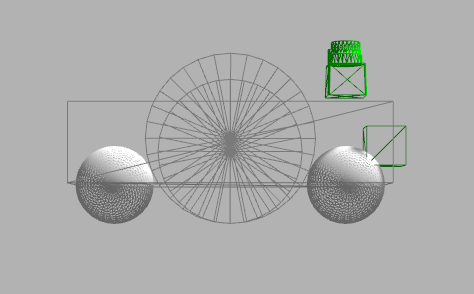
\includegraphics[scale=0.33]{udacity-design-2}
\caption{Udacity design view.}
\label{fig:mesh1}
\end{figure}

\begin{itemize}
\item Chassis: a box of size 40cm x 20cm x 1cm.
\item Wheels: two wheels 1cm x 0.5cm located in the front of the platform.
\item Casters: two caster one the back and another on the front.
\item Lidar: a hokuyo lidar in the front.
\item Camera: camera in the head of the platform
\end{itemize}


\subsection{Personal Model}

\subsubsection{Model design}

The model built from scratch consists in a 2W robot with a caster in the back to stabilise. A Lidar and a camera were added at the front, for the navigation stack. The inertial and friction parameters where adjusted in order to give a smooth movement to the robot.

\begin{figure}[h]
\centering
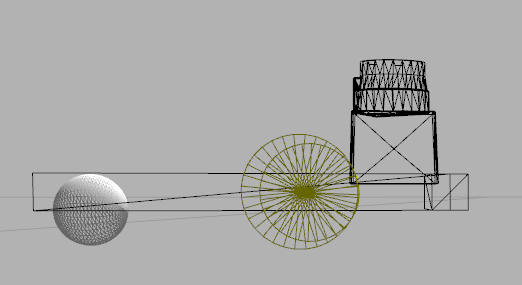
\includegraphics[scale=0.3]{robokoko-design-2}
\caption{Robokoko design view.}
\label{fig:mesh2}
\end{figure}

\begin{itemize}
\item Chassis: a box of size 22cm x 10cm x 2cm.
\item Wheels: two wheels 0.3cm x 0.3cm located in the front of the platform.
\item Back caster: one back caster in the back of the platform.
\item Lidar: a hokuyo lidar in the front.
\item Camera: camera in the front.
\end{itemize}

\subsection{Packages Used}

\begin{itemize}
\item gazebo: an application to simulate robots and the environment.
\item gazebo\_ros: this package provides a collection of plugins that allows ROS to interact with Gazebo by using services and topics.
\item rviz: it is a completely 3D visualization tool for ROS. It can subscribe to wide range of topic types to evaluate the performance of the solution.
\item map\_server: it offers map data as a ROS service.
\item tf: a package to keep track of multiple coordinate frames over time. It maintains the relationship between coordinate frames in a tree structure buffered in time.
\item amcl: a probabilistic localization system for a robot moving in 2D. It implements the Adaptive Monte Carlo localization algorithm.
\item move\_base: given a goal in the world will attempt to reach it with a mobile base. It links together a global and local planer, for the short-term and long-term planer respectively. In addition, it has got two costmaps, one for each planner, to generate n occupancy grid of the scene.
\end{itemize}

\subsection{Parameters}

\subsubsection{Localization parameters}

The following configuration parameters were chosen due to power limitations of the computer where packages were deployed, increasing this values may produced a better performance.

\begin{itemize}
\item min\_particles[1000]: Minimum allowed number of particles spread around the scene.
\item max\_particles[6000]: Maximum allowed number of particles spread around the scene. 
\item transform\_tolerance[0.5]: It is used to make a transformation valid in the future in order to cover lag in the system. Reducing this value improve performance but it is necessary to have computer power enough.
\item gui\_publish\_rate[1]: Maximum rate (Hz) at which scans and paths are published for visualization.
\end{itemize}

Parameters related to how recovering from stuck:

\begin{itemize}
\item recovery\_alpha\_slow[0.001]: Exponential decay rate for the slow average weight filter, used in deciding when to recover by adding random poses.   
\item recovery\_alpha\_fast[0.1]: Exponential decay rate for the fast average weight filter, 
used in deciding when to recover by adding random poses.
\end{itemize}

The following parameters give and estimation of the initial pose, mean and covariance, of the robot in the world, previous to any movement:

\begin{itemize}
\item initial\_pose\_x[0.0]: Initial pose mean (x), used to initialize filter with Gaussian distribution.
\item initial\_pose\_y[0.0]: Initial pose mean (y), used to initialize filter with Gaussian distribution.
\item initial\_pose\_a[0.0]: Initial pose mean (yaw), used to initialize filter with Gaussian distribution.
\item initial\_cov\_xx[0.25]: Initial pose covariance (x*x), used to initialize filter with Gaussian distribution.
\item initial\_cov\_yy[0.25]: Initial pose covariance (y*y), used to initialize filter with Gaussian distribution.
\item initial\_cov\_aa[0.07]: Initial pose covariance (yaw*yaw), used to initialize filter with Gaussian distribution.
\end{itemize}

Parameters related to the Laser and model configuration:

\begin{itemize}
\item laser\_likelihood\_max\_dist[2.0]: Maximum distance to do obstacle inflation on map, for use in likelihood\_field model.
\item laser\_model\_type[likelihood\_field]: Which model to use, either beam, likelihood\_field.
\item odom\_model\_type[diff\-corrected]: Which model to use, either "diff", "omni", "diff-corrected" or "omni-corrected". In our case the robot is diff type, the corrected include a bug correction.
\end{itemize}

The following parameters are about the noise in odemotry measurement. Because we are using a Bayesian Filter the probability of true values of odometry can be tuned using these parameters. These values where obtained by trail and error.

\begin{itemize}
\item odom\_alpha1[0.005]: Specifies the expected noise in odometry's rotation estimate from the rotational component of the robot's motion.
\item odom\_alpha2[0.005]: Specifies the expected noise in odometry's rotation estimate from translational component of the robot's motion. 
\item odom\_alpha3[0.010]: Specifies the expected noise in odometry's translation estimate from the translational component of the robot's motion. 
\item odom\_alpha4[0.010]: Specifies the expected noise in odometry's translation estimate from the rotational component of the robot's motion.
\end{itemize}

Parameters to configure the different frames names.

\begin{itemize}
\item odom\_frame\_id[odom]: Which frame to use for odometry.
\item base\_frame\_id[robot\_footprint]: Which frame to use for the robot base.
\item global\_frame\_id[map]: The name of the coordinate frame published by the localization system.
\end{itemize}

\subsubsection{Move base parameters}

The navigation stack uses cost-maps to store information about the obstacles in the world.


Costmap common parameters:

\begin{itemize}
\item obstacle\_range[2.5]: The robot will only update its map with information about obstacles that are within 2.5 meters of the base.
\item raytrace\_range[3.0]: This parameter determines the range to which we will raytrace freespace given a sensor reading. The robot will attempt to clear out space in front of it up to 3.0 meters away given a sensor reading.
\item robot\_radius[0.11]: The robot radius is 11cm. It's used to avoid passing the robot through narrow places where it can get stuck.
\item inflation\_radius[0.2]: The robot will treat all paths that stay 0.2 meters or more away from obstacles as having equal obstacle cost.
\item observation\_sources[laser\_scan\_sensor]: defines a list of sensors that are going to be passing information to the costmap. 
\item laser\_scan\_sensor[sensor\_frame: hokuyo, data\_type: LaserScan, topic: \/robokoko\/laser\/scan, marking: true, clearing: true]: gives the details about the previous observation source.
\end{itemize}

The local costmap is used by the local planner to generate a short-term plan. The local costmap uses the odometry information rather than a map.

In order to insert data from sensor sources into the costmap an extensive use of tf is used. Specifically, it assumes that all transforms between the coordinate frames specified by the global\_frame parameter, the robot\_base\_frame parameter, and sensor sources are connected. 

\begin{itemize}
\item global\_frame[odom]: The global frame for the costmap to operate in.
\item robot\_base\_frame[robot\_footprint]: The name of the frame for the base link of the robot.
\item update\_frequency[2]: The frequency, in Hz, at which the cost-map will run its update loop. 
\item publish\_frequency[2]: The rate, in Hz, at which the cost-map will publish visualization information.
\item width[20.0]: The cost-map's width.
\item height[20.0]: The cost-map's height.
\item resolution[0.05]: The cost-map's resolution.
\item static\_map[false]: The costmap should not initialize itself based on a map served by the map\_server, for the local costmap the odometry is used.
\item rolling\_window[true]:  the robot only cares about obstacles within a local area.
\item transform\_tolerance[0.5]: Specifies the delay in transform (tf) data that is tolerable in seconds.
\end{itemize}

The global costmap is used by the local planner to generate a long-term plan. The global costmap uses the map provided by the map\_server.

\begin{itemize}
\item global\_frame[map]: The global frame for the costmap to operate in.
\item robot\_base\_frame[robot\_footprint]: The name of the frame for the base link of the robot. 
\item update\_frequency[2]: The frequency, in Hz, at which the cost-map will run its update loop. 
\item publish\_frequency[2]: The rate, in Hz, at which the cost-map will publish visualization information.
\item width[40.0]: The cost-map's width.
\item height[40.0]:The cost-map's height.
\item resolution[0.05]: The cost-map's resolution.
\item static\_map[true]: The costmap should initialize itself based on a map served by the map\_server.
\item rolling\_window[false]: for global localization this parameter must set to false.
\item transform\_tolerance[0.5]: Specifies the delay in transform (tf) data that is tolerable in seconds. 
\end{itemize}

This package provides implementations of the Trajectory Rollout and Dynamic Window approaches to local robot navigation on a plane. Given a plan to follow and a costmap, the controller produces velocity commands to send to the robot.

\begin{itemize}
\item holonomic\_robot[false]: Determines whether velocity commands are generated for a holonomic or non-holonomic robot. Our model is not holonomic.
\item sim\_time[2.0]: The amount of time to forward-simulate trajectories in seconds. This values was selected due to computer power restrictions.
\item meter\_scoring[true]: Whether the gdist\_scale and pdist\_scale parameters should assume that goal\_distance and path\_distance are expressed in units of meters or cells.
\item max\_vel\_x[0.4]: The maximum forward velocity allowed for the base in meters/sec.
\item min\_vel\_x[0.1]: The minimum forward velocity allowed for the base in meters/sec.
\item max\_vel\_theta[0.7]: The maximum rotational velocity allowed for the base in radians/sec.
\item min\_vel\_theta[-0.7]: The minimum rotational velocity allowed for the base in radians/sec.
\item acc\_lim\_x[0.6]: The x acceleration limit of the robot in meters/sec$^2$.
\item acc\_lim\_y[0.6]: The y acceleration limit of the robot in meters/sec$^2$.
\item acc\_lim\_theta[1.5]: The rotational acceleration limit of the robot in radians/sec$^2$.
\end{itemize}

\section{Results}

In the first part of the project the robot model was created and an initial set-up of the packages was defined. In order to check how far the configuration was from the final solution, small demands to the robot's pose were sent using Rviz navigation tools.

This was the approaches used in order to get the final result:
\begin{enumerate}
\item The correct odometry of the robot was checked by sending basic commands, without amcl package in execution, to move: forward, backward an in circles. The inertial and friction parameters were adjusted in the robot model to avoid erratic movements. 
\item Some parameters related to the computer power limitation were adjusted in order to solve control loop problems: number of particles, transform tolerances, update and publish frequencies.
\item The robot was sent to the final goal position. The amcl parameters related to the odometry, the costmap parameters related to the inflation, robot radios were adjusted in order to navigate smoohtly, without getting stuck and detecting correctly the obstacles.  
\end{enumerate}	

\subsection{Localization Results}
\subsubsection{Benchmark}

After adjusting these parameters the udacity robot was able to get to the goal position in a reasonable time, two minutes approximately. Two minutes is  good solution taking into account the limitation and dead lines of the project. A finer adjustment of the parameters can probably give a better solution, less than a minute.. The particles filter converges in few second, this can be visualized using the rviz tool and the robot follows a smooth path to the goal. The experiment was repeated several times and in some occasions the robot get stuck in the corners of the obstacles in the map. 

\begin{figure}[h]
\centering
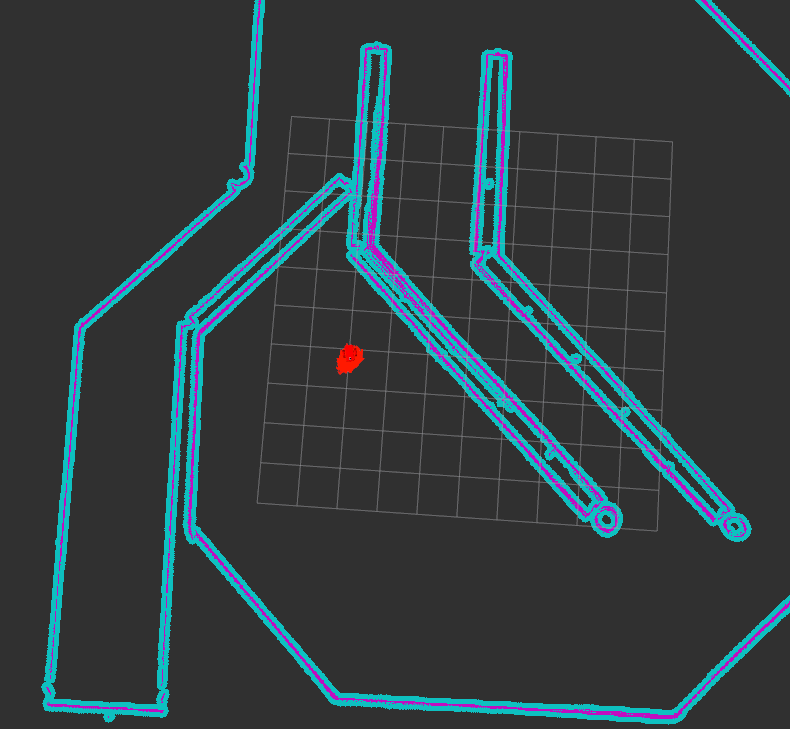
\includegraphics[scale=0.25]{rviz-robot-udacity-goal-position}
\caption{Udacity final goal position}
\label{fig:mesh3}
\end{figure}

\subsubsection{Student}

Similar result was obtained by the robokoko robot. The particle filter converges, the robot follows a smooth path and the robot goes to the goal position.

\begin{figure}[h]
\centering
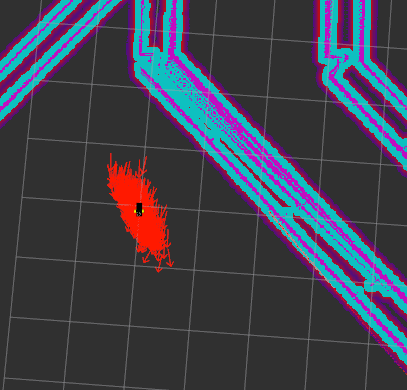
\includegraphics[scale=0.3]{rviz-robot-own-goal-position}
\caption{Robokoko final goal position}
\label{fig:mesh4}
\end{figure}

\subsection{Technical Comparison} % only facts

The robokoko robot is quite similar to the udacity robot. The main difference is that the robokoko robot is lighter. This allows the robot to move quicker. The same parameters were used for both the udacity and robokoko robots. 

\section{Discussion}

Even the robot is able to go to the final position in a reasonable time I have found two problems that have space for improvement:

\begin{enumerate}
\item Sometime the head of the robot swings producing the Lidar to measure the floor as an obstacle. The back caster weight was increased and the acceleration maximum and minimum was reduced. This still happens from time to time and it produces the effect to identify as obstacle the floor by the local planner. More research is necessary.
\item There are some parameters in the local planner, related to the cost-map, that are producing the robot to get stuck in the corners of the obstacles from time to time. The robot recover from this situation but a it is necessary to investigate a more robust solution.
\end{enumerate}	

\subsection{Topics}

\begin{itemize}
\item After several test we can get the conclusion that both robots performance similarly.
\item The robokoko is a little bit quicker due to its lightness.
\item The AMCL localization can be used in scenarios where we have a map of the scene as for example for the robot to guide in a museum.
\item The AMCL localization solutions can be used in the industrial domain to different kind of applications: smart robot to clean the floors, to carry out heavy loads, for entertainment etc...
\item  In order to resolve the kidnapped problem using AMCL two problems must be overcome: the kidnapped robot must be detected and them there must be a way to recover.  The kidnapped event can be detected based on robot’s sensor reading and the displacement  between two consecutive reading \cite{kidnapped}.  In addition, the recover from the kidnapped problem a feature matching strategy can be used marking the scene with some fiducial markers.\cite{kidnappedrecover} 
\end{itemize}

\section{Conclusion / Future work}


During this project a model of a robot has been built from scratch. All the parameters related to dimensions, mass, inertia and friction values have been set as much realistic as possible. Then, the amlc and navigation stack have been configured. All the more significant parameters have been adjusted in order to achieve a reasonable performance. As result, the robot can achieve the target position in a reasonable amount of time. 

In order to obtain a better performance there are several things that can be done. The model can be optimized to provide to the robot more velocity. The parameters can be futher optimized to get to the goal in a shorter time. This work has not been done due a time restrictions, the project has got a dead line.

Finally, it has been observed some limitations about the hardware where the solution was deployed. A analysis to define the hardware requirement should be done if the solution is intented to deploy in a real system.

This solution can be adapted to be the base for a real application. For instance, a guide robot for a museum or the guide robot for the Gran Telescopio Canarias, the place where I work.

\begin{thebibliography}{9}
\bibliographystyle{ieeetr}

\bibitem{probabilisticrobotics} 
Sebastian Thrun, Wolfram Burgard, and Dieter Fox
\textit{Probabilistic Robotics}. 

\bibitem{robustmontecarlo} 
Sebastian Thrun, Dieter Fox , Wolfram Burgard , and Frank Dellaert
\textit{Robust Monte Carlo Localization for Mobile Robots}. 

\bibitem{udacity} 
https://eu.udacity.com
\textit{Robotics Software Engineer Nanodegree program}. 

\bibitem{kidnapped} 
Iksan Bukhori and Zool Hilmi Ismail
\textit{Detection of kidnapped robot problem in Monte Carlo localization based on the natural displacement of the robot}. 

\bibitem{kidnappedrecover} 
Lei Wei
\textit{A Feature-based Solution for Kidnapped Robot Problem}. 



\end{thebibliography}
\end{document}
